\section{Results}
\label{sec:results}
% \subsection{Description}
% This section presents the results of your experiments,
% comparing your solution to other schemes. The metrics of
% interest are highly dependent on the topic of research, but
% should optimally cover all interesting aspects of your scheme.
% Informative graphs or tables are the key to a good result
% section.
% Furthermore, you need to discuss your results. You should
% give explanations of distinctive points and outliers in your
% results. It is also necessary to state why your scheme is
% better/worse compared to the other schemes. Thus, this section
% consists of two parts: the results of your experiments, as well
% as an explanation as to why the results are as they are
%
\subsubsection{Sequential Prefetcher}
During the early stages of development a naive implementation of a prefetcher was tested.
The resulting speedup for different prefetching degrees can be seen in Figure \ref{fig:sequential}.
From the Figure one can determine that a sequential prefetcher with a degree of 3 yielded best results.

This prefetcher yields great speedup for the applu benchmark, but has a significant negative impact on the ammp benchmark.

\begin{figure*}
    \label{fig:sequential}
    % GNUPLOT: LaTeX picture with Postscript
\begingroup
  \makeatletter
  \providecommand\color[2][]{%
    \GenericError{(gnuplot) \space\space\space\@spaces}{%
      Package color not loaded in conjunction with
      terminal option `colourtext'%
    }{See the gnuplot documentation for explanation.%
    }{Either use 'blacktext' in gnuplot or load the package
      color.sty in LaTeX.}%
    \renewcommand\color[2][]{}%
  }%
  \providecommand\includegraphics[2][]{%
    \GenericError{(gnuplot) \space\space\space\@spaces}{%
      Package graphicx or graphics not loaded%
    }{See the gnuplot documentation for explanation.%
    }{The gnuplot epslatex terminal needs graphicx.sty or graphics.sty.}%
    \renewcommand\includegraphics[2][]{}%
  }%
  \providecommand\rotatebox[2]{#2}%
  \@ifundefined{ifGPcolor}{%
    \newif\ifGPcolor
    \GPcolorfalse
  }{}%
  \@ifundefined{ifGPblacktext}{%
    \newif\ifGPblacktext
    \GPblacktexttrue
  }{}%
  % define a \g@addto@macro without @ in the name:
  \let\gplgaddtomacro\g@addto@macro
  % define empty templates for all commands taking text:
  \gdef\gplbacktext{}%
  \gdef\gplfronttext{}%
  \makeatother
  \ifGPblacktext
    % no textcolor at all
    \def\colorrgb#1{}%
    \def\colorgray#1{}%
  \else
    % gray or color?
    \ifGPcolor
      \def\colorrgb#1{\color[rgb]{#1}}%
      \def\colorgray#1{\color[gray]{#1}}%
      \expandafter\def\csname LTw\endcsname{\color{white}}%
      \expandafter\def\csname LTb\endcsname{\color{black}}%
      \expandafter\def\csname LTa\endcsname{\color{black}}%
      \expandafter\def\csname LT0\endcsname{\color[rgb]{1,0,0}}%
      \expandafter\def\csname LT1\endcsname{\color[rgb]{0,1,0}}%
      \expandafter\def\csname LT2\endcsname{\color[rgb]{0,0,1}}%
      \expandafter\def\csname LT3\endcsname{\color[rgb]{1,0,1}}%
      \expandafter\def\csname LT4\endcsname{\color[rgb]{0,1,1}}%
      \expandafter\def\csname LT5\endcsname{\color[rgb]{1,1,0}}%
      \expandafter\def\csname LT6\endcsname{\color[rgb]{0,0,0}}%
      \expandafter\def\csname LT7\endcsname{\color[rgb]{1,0.3,0}}%
      \expandafter\def\csname LT8\endcsname{\color[rgb]{0.5,0.5,0.5}}%
    \else
      % gray
      \def\colorrgb#1{\color{black}}%
      \def\colorgray#1{\color[gray]{#1}}%
      \expandafter\def\csname LTw\endcsname{\color{white}}%
      \expandafter\def\csname LTb\endcsname{\color{black}}%
      \expandafter\def\csname LTa\endcsname{\color{black}}%
      \expandafter\def\csname LT0\endcsname{\color{black}}%
      \expandafter\def\csname LT1\endcsname{\color{black}}%
      \expandafter\def\csname LT2\endcsname{\color{black}}%
      \expandafter\def\csname LT3\endcsname{\color{black}}%
      \expandafter\def\csname LT4\endcsname{\color{black}}%
      \expandafter\def\csname LT5\endcsname{\color{black}}%
      \expandafter\def\csname LT6\endcsname{\color{black}}%
      \expandafter\def\csname LT7\endcsname{\color{black}}%
      \expandafter\def\csname LT8\endcsname{\color{black}}%
    \fi
  \fi
  \setlength{\unitlength}{0.0500bp}%
  \begin{picture}(10204.00,2834.00)%
    \gplgaddtomacro\gplbacktext{%
      \csname LTb\endcsname%
      \put(946,704){\makebox(0,0)[r]{\strut{} 0.5}}%
      \put(946,970){\makebox(0,0)[r]{\strut{} 0.6}}%
      \put(946,1237){\makebox(0,0)[r]{\strut{} 0.7}}%
      \put(946,1503){\makebox(0,0)[r]{\strut{} 0.8}}%
      \put(946,1770){\makebox(0,0)[r]{\strut{} 0.9}}%
      \put(946,2036){\makebox(0,0)[r]{\strut{} 1}}%
      \put(946,2303){\makebox(0,0)[r]{\strut{} 1.1}}%
      \put(946,2569){\makebox(0,0)[r]{\strut{} 1.2}}%
      \put(1518,484){\makebox(0,0){\strut{} 1}}%
      \put(2398,484){\makebox(0,0){\strut{} 2}}%
      \put(3277,484){\makebox(0,0){\strut{} 3}}%
      \put(4157,484){\makebox(0,0){\strut{} 4}}%
      \put(5037,484){\makebox(0,0){\strut{} 5}}%
      \put(5916,484){\makebox(0,0){\strut{} 6}}%
      \put(6796,484){\makebox(0,0){\strut{} 7}}%
      \put(176,1636){\rotatebox{-270}{\makebox(0,0){\strut{}Speedup}}}%
      \put(4157,154){\makebox(0,0){\strut{}Prefetching degree}}%
    }%
    \gplgaddtomacro\gplfronttext{%
      \csname LTb\endcsname%
      \put(9216,2459){\makebox(0,0)[r]{\strut{}ammp}}%
      \csname LTb\endcsname%
      \put(9216,2239){\makebox(0,0)[r]{\strut{}applu}}%
      \csname LTb\endcsname%
      \put(9216,2019){\makebox(0,0)[r]{\strut{}apsi}}%
      \csname LTb\endcsname%
      \put(9216,1799){\makebox(0,0)[r]{\strut{}art110}}%
      \csname LTb\endcsname%
      \put(9216,1579){\makebox(0,0)[r]{\strut{}art470}}%
      \csname LTb\endcsname%
      \put(9216,1359){\makebox(0,0)[r]{\strut{}bzip2-graphic}}%
      \csname LTb\endcsname%
      \put(9216,1139){\makebox(0,0)[r]{\strut{}bzip2-program}}%
    }%
    \gplbacktext
    \put(0,0){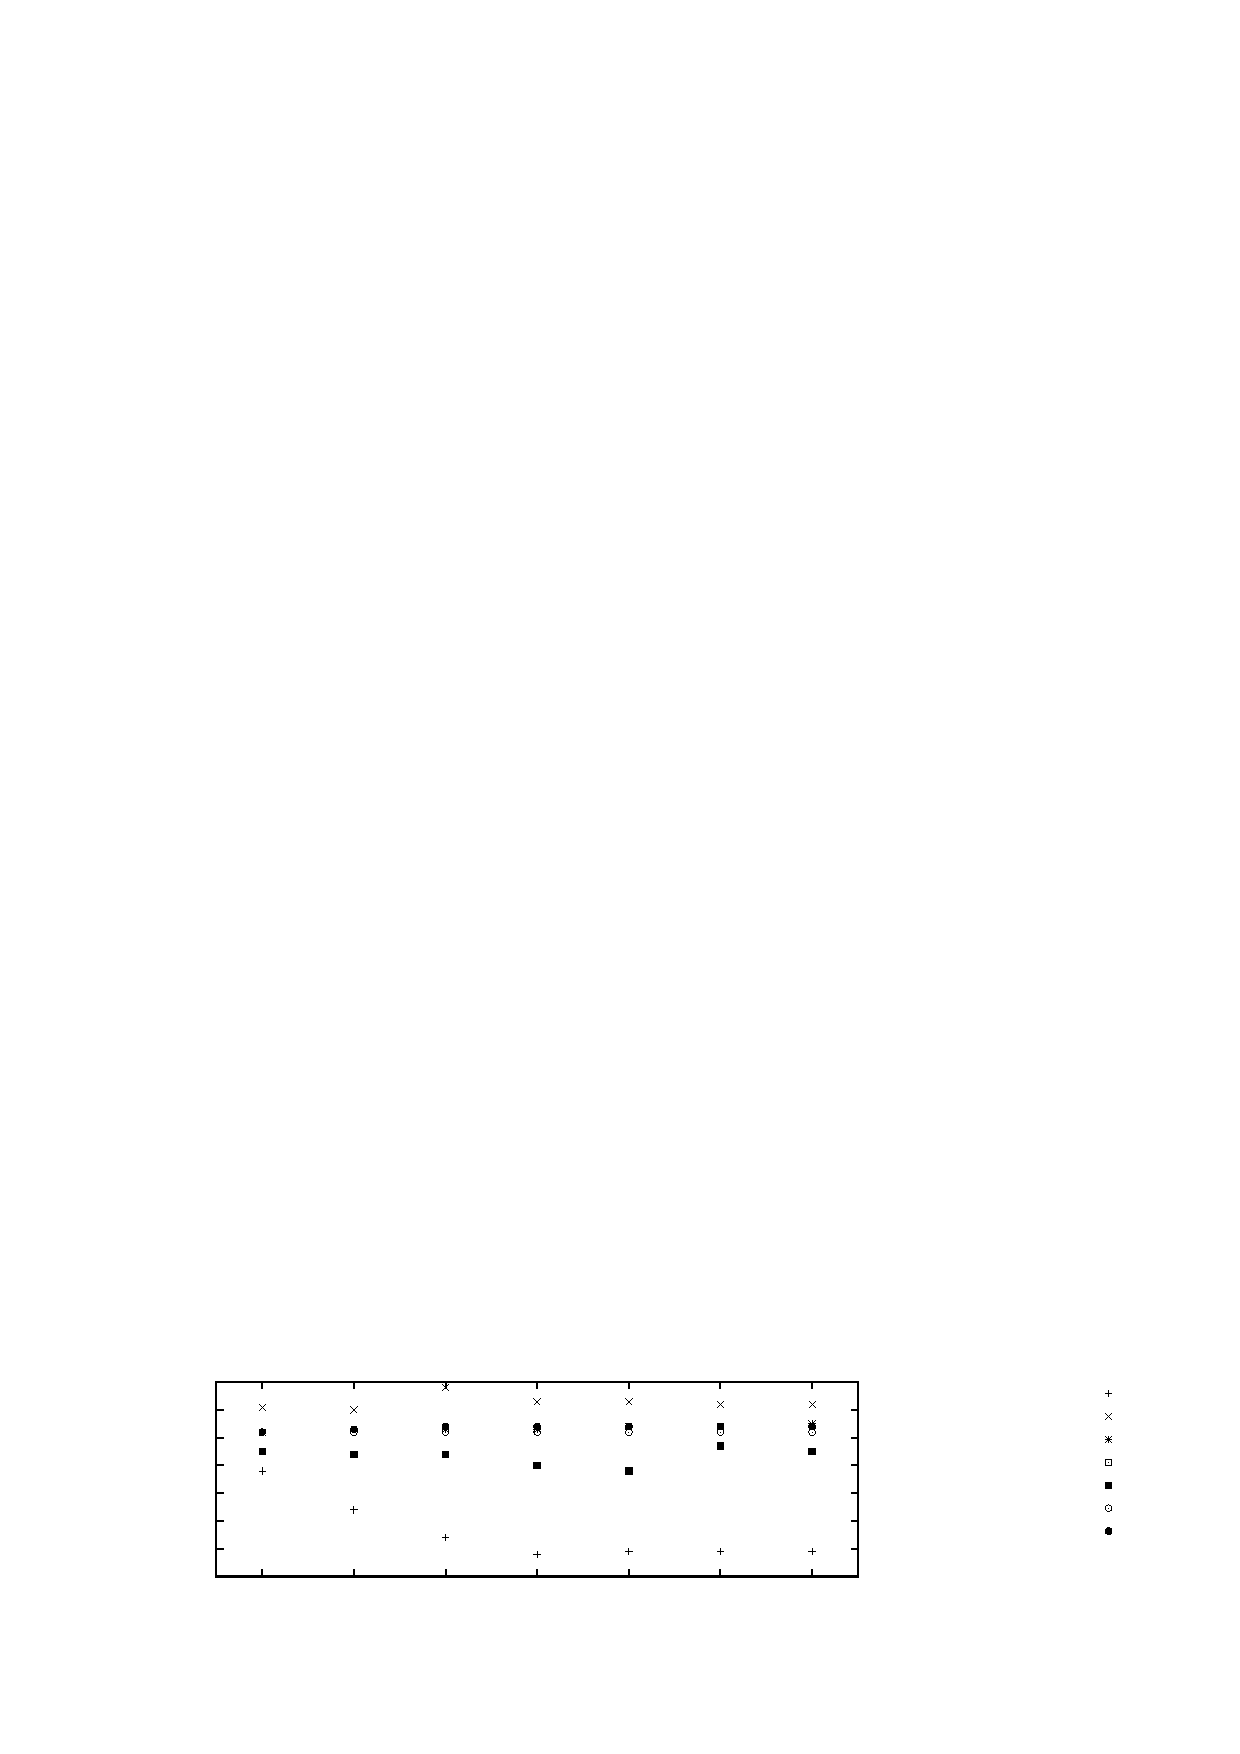
\includegraphics{plots/sequential}}%
    \gplfronttext
  \end{picture}%
\endgroup

    \caption{Speedup of each benchmark as a function of degree for the sequential prefetcher.}
\end{figure*}



\subsubsection{Stride Direct Prefetcher}
(todo)

\subsubsection{Reference Table Prefetcher}
(todo)


\subsubsection{Global History Buffer with Delta Correlation}
The implementation of the global history buffer with SDP and RTP as fallback was successfully implemented and yielded the speedups shown in Figure \ref{fig:ghbdc}.
The best speedup was acquired for the ammp benchmark, but many of the other benchmark showed only a slight speedup if any at all.



\begin{figure*}
    \label{fig:ghbdc}
    % GNUPLOT: LaTeX picture with Postscript
\begingroup
  \makeatletter
  \providecommand\color[2][]{%
    \GenericError{(gnuplot) \space\space\space\@spaces}{%
      Package color not loaded in conjunction with
      terminal option `colourtext'%
    }{See the gnuplot documentation for explanation.%
    }{Either use 'blacktext' in gnuplot or load the package
      color.sty in LaTeX.}%
    \renewcommand\color[2][]{}%
  }%
  \providecommand\includegraphics[2][]{%
    \GenericError{(gnuplot) \space\space\space\@spaces}{%
      Package graphicx or graphics not loaded%
    }{See the gnuplot documentation for explanation.%
    }{The gnuplot epslatex terminal needs graphicx.sty or graphics.sty.}%
    \renewcommand\includegraphics[2][]{}%
  }%
  \providecommand\rotatebox[2]{#2}%
  \@ifundefined{ifGPcolor}{%
    \newif\ifGPcolor
    \GPcolorfalse
  }{}%
  \@ifundefined{ifGPblacktext}{%
    \newif\ifGPblacktext
    \GPblacktexttrue
  }{}%
  % define a \g@addto@macro without @ in the name:
  \let\gplgaddtomacro\g@addto@macro
  % define empty templates for all commands taking text:
  \gdef\gplbacktext{}%
  \gdef\gplfronttext{}%
  \makeatother
  \ifGPblacktext
    % no textcolor at all
    \def\colorrgb#1{}%
    \def\colorgray#1{}%
  \else
    % gray or color?
    \ifGPcolor
      \def\colorrgb#1{\color[rgb]{#1}}%
      \def\colorgray#1{\color[gray]{#1}}%
      \expandafter\def\csname LTw\endcsname{\color{white}}%
      \expandafter\def\csname LTb\endcsname{\color{black}}%
      \expandafter\def\csname LTa\endcsname{\color{black}}%
      \expandafter\def\csname LT0\endcsname{\color[rgb]{1,0,0}}%
      \expandafter\def\csname LT1\endcsname{\color[rgb]{0,1,0}}%
      \expandafter\def\csname LT2\endcsname{\color[rgb]{0,0,1}}%
      \expandafter\def\csname LT3\endcsname{\color[rgb]{1,0,1}}%
      \expandafter\def\csname LT4\endcsname{\color[rgb]{0,1,1}}%
      \expandafter\def\csname LT5\endcsname{\color[rgb]{1,1,0}}%
      \expandafter\def\csname LT6\endcsname{\color[rgb]{0,0,0}}%
      \expandafter\def\csname LT7\endcsname{\color[rgb]{1,0.3,0}}%
      \expandafter\def\csname LT8\endcsname{\color[rgb]{0.5,0.5,0.5}}%
    \else
      % gray
      \def\colorrgb#1{\color{black}}%
      \def\colorgray#1{\color[gray]{#1}}%
      \expandafter\def\csname LTw\endcsname{\color{white}}%
      \expandafter\def\csname LTb\endcsname{\color{black}}%
      \expandafter\def\csname LTa\endcsname{\color{black}}%
      \expandafter\def\csname LT0\endcsname{\color{black}}%
      \expandafter\def\csname LT1\endcsname{\color{black}}%
      \expandafter\def\csname LT2\endcsname{\color{black}}%
      \expandafter\def\csname LT3\endcsname{\color{black}}%
      \expandafter\def\csname LT4\endcsname{\color{black}}%
      \expandafter\def\csname LT5\endcsname{\color{black}}%
      \expandafter\def\csname LT6\endcsname{\color{black}}%
      \expandafter\def\csname LT7\endcsname{\color{black}}%
      \expandafter\def\csname LT8\endcsname{\color{black}}%
    \fi
  \fi
  \setlength{\unitlength}{0.0500bp}%
  \begin{picture}(10204.00,2834.00)%
    \gplgaddtomacro\gplbacktext{%
      \csname LTb\endcsname%
      \put(946,704){\makebox(0,0)[r]{\strut{} 1}}%
      \put(946,970){\makebox(0,0)[r]{\strut{} 1.1}}%
      \put(946,1237){\makebox(0,0)[r]{\strut{} 1.2}}%
      \put(946,1503){\makebox(0,0)[r]{\strut{} 1.3}}%
      \put(946,1770){\makebox(0,0)[r]{\strut{} 1.4}}%
      \put(946,2036){\makebox(0,0)[r]{\strut{} 1.5}}%
      \put(946,2303){\makebox(0,0)[r]{\strut{} 1.6}}%
      \put(946,2569){\makebox(0,0)[r]{\strut{} 1.7}}%
      \put(1518,484){\makebox(0,0){\strut{} 1}}%
      \put(2398,484){\makebox(0,0){\strut{} 2}}%
      \put(3277,484){\makebox(0,0){\strut{} 3}}%
      \put(4157,484){\makebox(0,0){\strut{} 4}}%
      \put(5037,484){\makebox(0,0){\strut{} 5}}%
      \put(5916,484){\makebox(0,0){\strut{} 6}}%
      \put(6796,484){\makebox(0,0){\strut{} 7}}%
      \put(176,1636){\rotatebox{-270}{\makebox(0,0){\strut{}Speedup}}}%
      \put(4157,154){\makebox(0,0){\strut{}Prefetching degree}}%
    }%
    \gplgaddtomacro\gplfronttext{%
      \csname LTb\endcsname%
      \put(9216,2459){\makebox(0,0)[r]{\strut{}ammp}}%
      \csname LTb\endcsname%
      \put(9216,2239){\makebox(0,0)[r]{\strut{}applu}}%
      \csname LTb\endcsname%
      \put(9216,2019){\makebox(0,0)[r]{\strut{}apsi}}%
      \csname LTb\endcsname%
      \put(9216,1799){\makebox(0,0)[r]{\strut{}art110}}%
      \csname LTb\endcsname%
      \put(9216,1579){\makebox(0,0)[r]{\strut{}art470}}%
      \csname LTb\endcsname%
      \put(9216,1359){\makebox(0,0)[r]{\strut{}bzip2-graphic}}%
      \csname LTb\endcsname%
      \put(9216,1139){\makebox(0,0)[r]{\strut{}bzip2-program}}%
    }%
    \gplbacktext
    \put(0,0){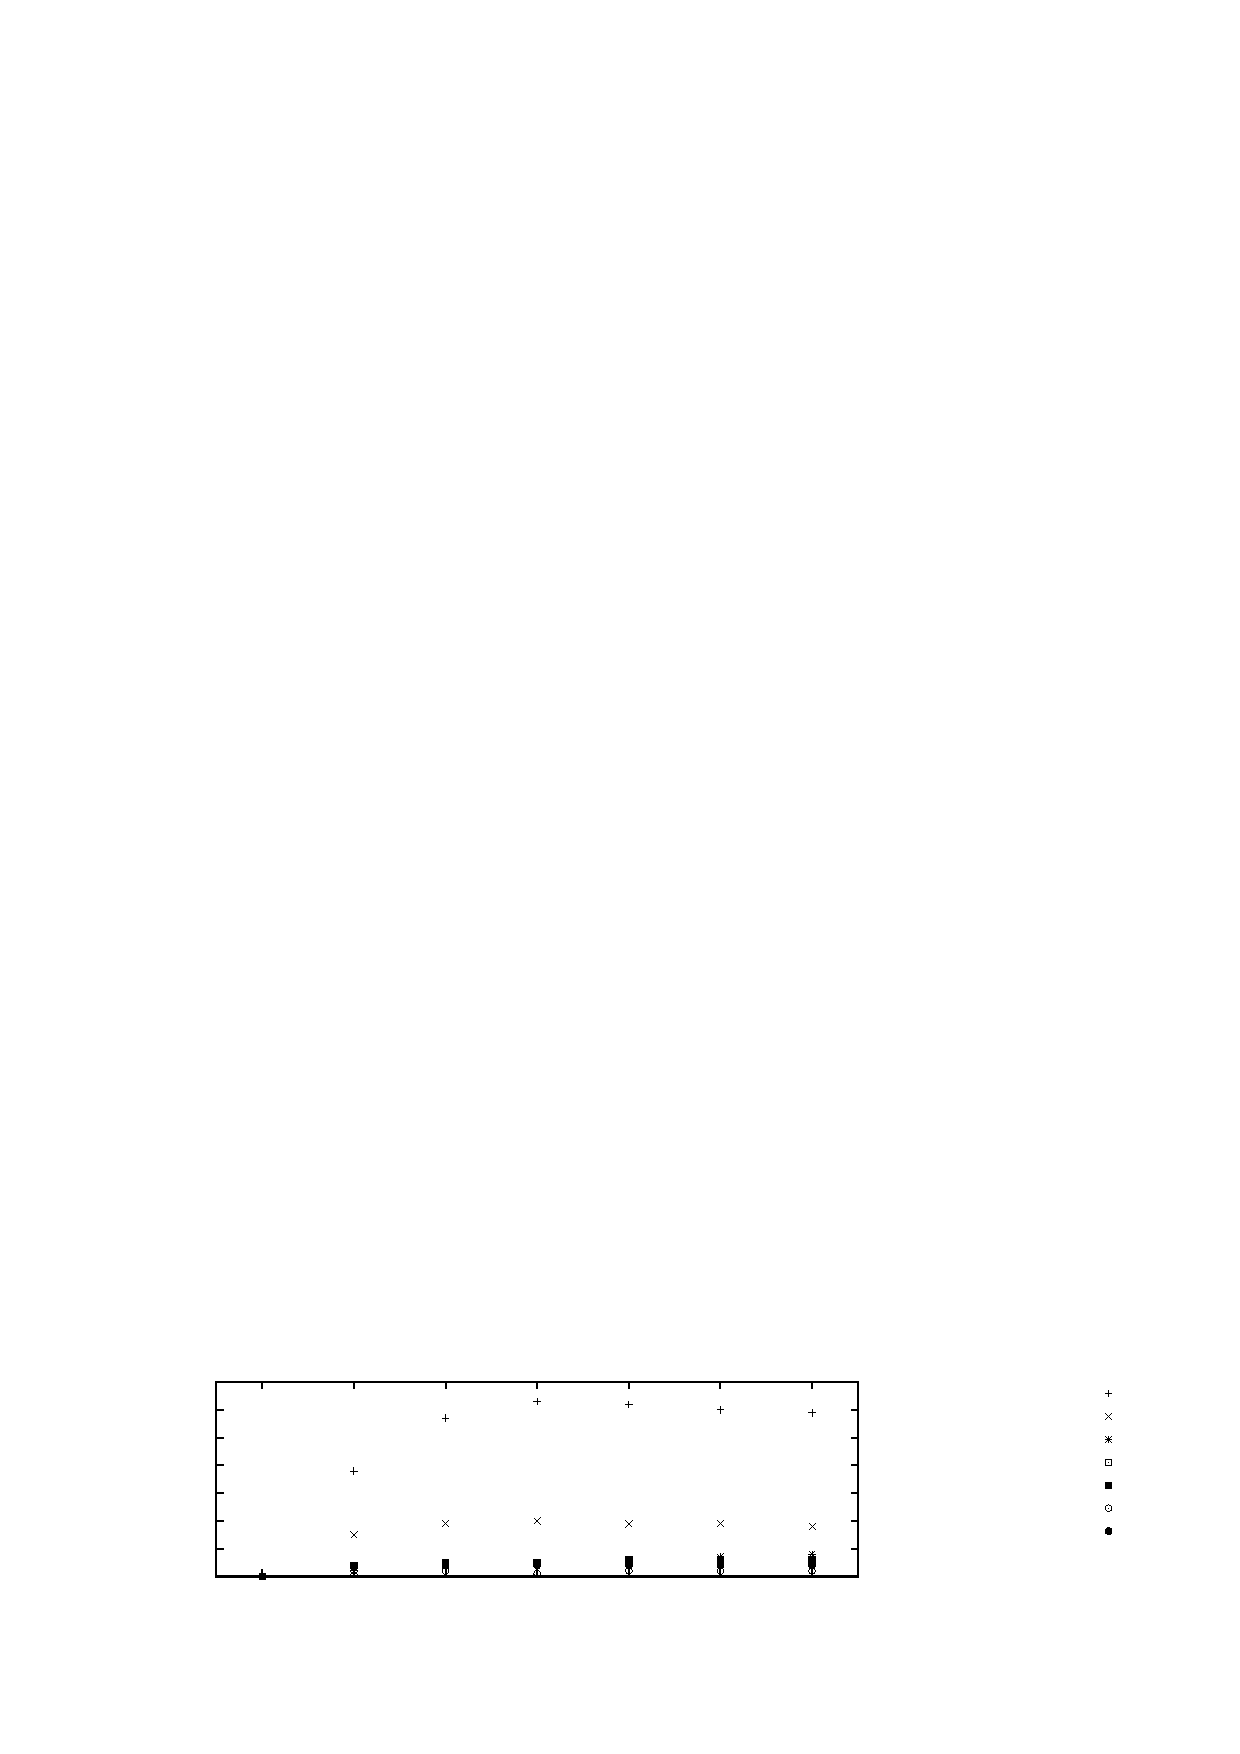
\includegraphics{plots/ghbdc}}%
    \gplfronttext
  \end{picture}%
\endgroup

    \caption{Speedup of each benchmark as a function of degree for the global history buffer with delta correlation and fall back to SDP and RTP.}
\end{figure*}
